
% Change the style for the front page, put in a background image.
\setbeamertemplate{background canvas}{%
%  \includegraphics[width=\paperwidth]{title-tip_2-dark}}
  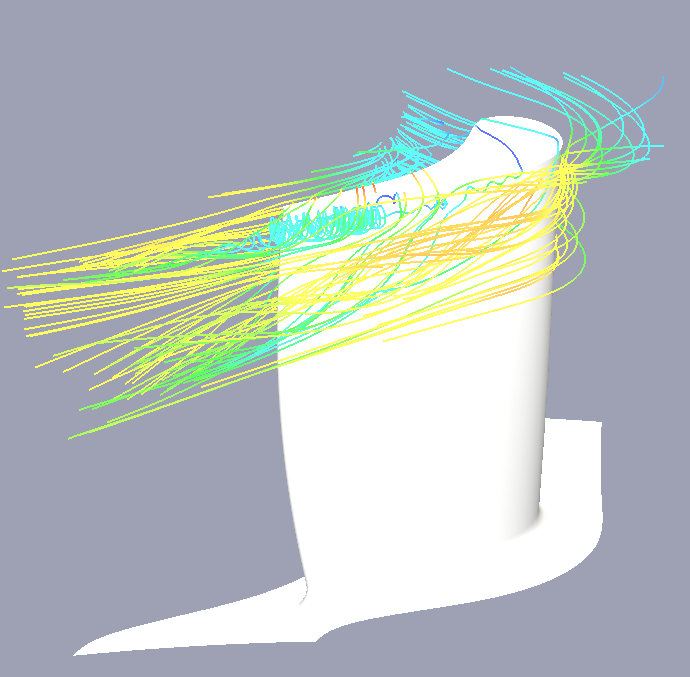
\includegraphics[width=\paperwidth]{title-tip_2-bright}}
%    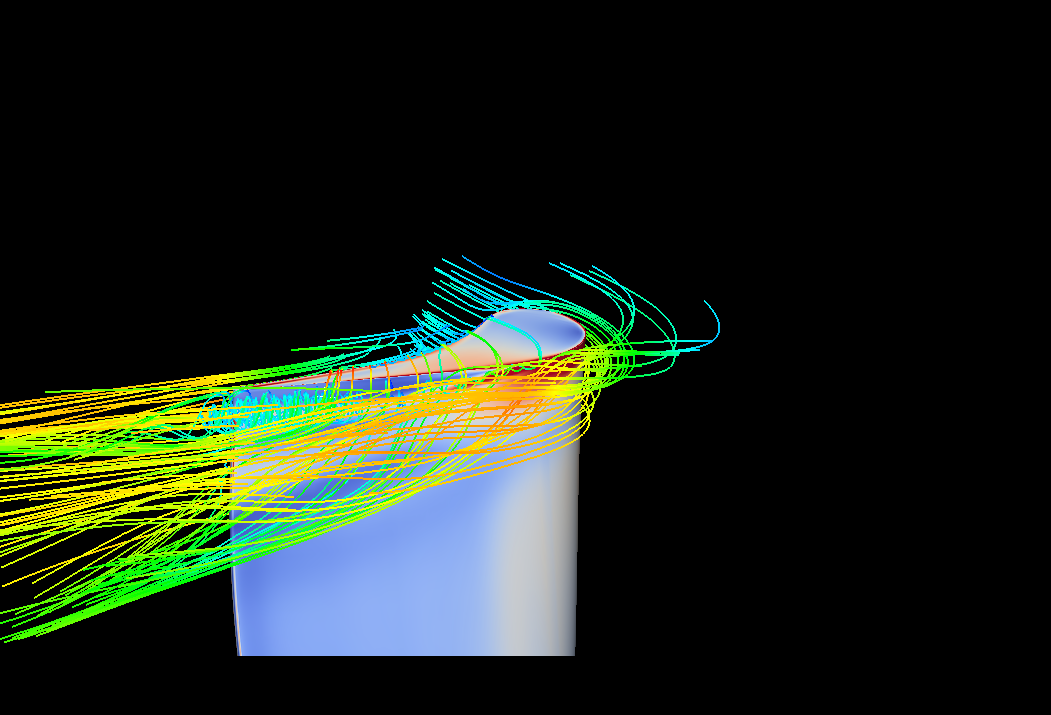
\includegraphics[width=14.2cm]{streamline7.png}}

\begin{frame}[plain]
  % titlepage; move things around to suit the image.
\vfill\vfill
\leftline{\color{black}\huge\bf Stabilization of a discrete adjoint}
\center{\color{black}\huge\bf using implicit time stepping}
\vfill\vfill
\vfill\vfill\vfill\vfill

\rightline{\color{black}\bf Sheikh Razibul Islam}
\rightline{\color{black}\bf Prof. Jacek Szumbarski}
\rightline{\color{black}\bf {Warsaw University of Technology}}
\rightline{\color{black}\bf {Poland}}

\vfill\vfill

\begin{columns}
  \begin{column}{.4\textwidth}
%    \includegraphics[width=\linewidth]{QM144BlueOnLight}
%   \includegraphics[width=\linewidth]{QM144WhiteOnDark}
%    
\includegraphics[width=\linewidth]{ccfd3}
%    
\includegraphics[scale=0.05]{logo_PW}

  \end{column}
  \begin{column}{.6\textwidth}
    \rightline{\color{black}\large \bf AboutFlow Midterm Review Meeting}
    \rightline{\color{black}\large \bf RWTH Aachen, 1 September 2014}    
  \end{column}

\end{columns}

\end{frame}
\setbeamertemplate{background canvas}[default]
